\documentclass[11pt,a4paper]{article}
\usepackage[utf8]{inputenc}
\usepackage[spanish,es-tabla]{babel}
\usepackage{amsmath,amssymb,amsfonts,mathtools,bm}
\usepackage{graphicx}
\usepackage{booktabs}
\usepackage{array}
\usepackage{geometry}
\usepackage{fancyhdr}
\usepackage{setspace}
\usepackage{titlesec}
\usepackage{caption}
\usepackage{enumitem}
\usepackage{hyperref}

% Márgenes Oficiales UNI (RR 1439-2023)
\geometry{
    a4paper,
    left=3.0cm,
    top=2.54cm,
    right=2.5cm,
    bottom=2.5cm,
    headheight=15pt,
    footskip=1.25cm
}

\setstretch{1.15}

\hypersetup{
    colorlinks=false,
    pdfborder={0 0 0}
}

\pagestyle{fancy}
\fancyhf{}
\renewcommand{\headrulewidth}{0.4pt}
\fancyhead[L]{\small\scshape UNIVERSIDAD NACIONAL DE INGENIERÍA | FIGMM}
\fancyhead[R]{\small\thepage}
\fancyfoot[C]{\small Trabajo de Investigación Técnica -- Gerencia Mina Cuajone 2025}

\titleformat{\section}{\normalfont\Large\bfseries}{\thesection.}{0.8em}{}
\titleformat{\subsection}{\normalfont\large\bfseries}{\thesubsection.}{0.6em}{}

\begin{document}

% PORTADA INSTITUCIONAL UNI (100% NEGRO)
\begin{titlepage}
    \centering
    {\bfseries\LARGE UNIVERSIDAD NACIONAL DE INGENIERÍA\par}
    \vspace{0.3cm}
    {\bfseries\large FACULTAD DE INGENIERÍA GEOLÓGICA, MINERA Y METALÚRGICA\par}
    \vspace{0.2cm}
    {\bfseries\large ESCUELA PROFESIONAL DE INGENIERÍA DE MINAS\par}
    \vspace{1.0cm}
    \hrule height 1.5pt
    \vspace{1.2cm}
    
    {\bfseries\Large INFORME DE INVESTIGACIÓN TÉCNICA OPERACIONAL\par}
    \vspace{1.2cm}
    
    {\bfseries\LARGE `PESAJE DE VOLQUETES GERENCIA MINA CUAJONE 2025''\par}
    \vspace{1.8cm}
    
    \begin{flushleft}
    \hspace{2.5cm}\textbf{\large ÁREA:}\\
    \hspace{2.5cm}{\normalsize Entrenamiento Mina / Operaciones Mina}\par
    \hspace{2.5cm}{\normalsize Superintendencia de Operaciones Mina Cuajone}\par
    \vspace{0.8cm}
    
    \hspace{2.5cm}\textbf{\large DIRIGIDO A:}\\
    \hspace{2.5cm}{\normalsize Superintendente de Operaciones Mina}\par
    \vspace{0.8cm}
    
    \hspace{2.5cm}\textbf{\large ELABORADO POR:}\\
    \hspace{2.5cm}{\normalsize Becario de Operaciones Mina}\par
    \vspace{0.8cm}
    
    \hspace{2.5cm}\textbf{\large FECHA DE ELABORACIÓN:}\\
    \hspace{2.5cm}{\normalsize 24 de Octubre del 2025}\par
    \end{flushleft}
    
    \vfill
    {\bfseries\large MOQUEGUA -- PERÚ\par}
    {\large 2025\par}
\end{titlepage}

\tableofcontents
\newpage

\section{RESUMEN}
\subsection{Alcances}
El 12 de octubre de 2025 se llevaron a cabo los trabajos finales de preparación en la zona de pesaje, los cuales comprendieron labores de relleno, nivelación y compactación del terreno. Para la ejecución de estas actividades se emplearon los equipos Cargador Frontal WA470 (F972), Motoniveladora CAT 24M (M244) y Rodillo Bomag WB 226 DH-5 (RCC-1). Asimismo, con el propósito de garantizar una mayor precisión en la nivelación del terreno, se contó con el apoyo técnico de la empresa contratista Mincoser. En las Figuras 1 y 2 se presentan los trabajos realizados durante esta etapa.

\begin{figure}[htbp]
    \centering
    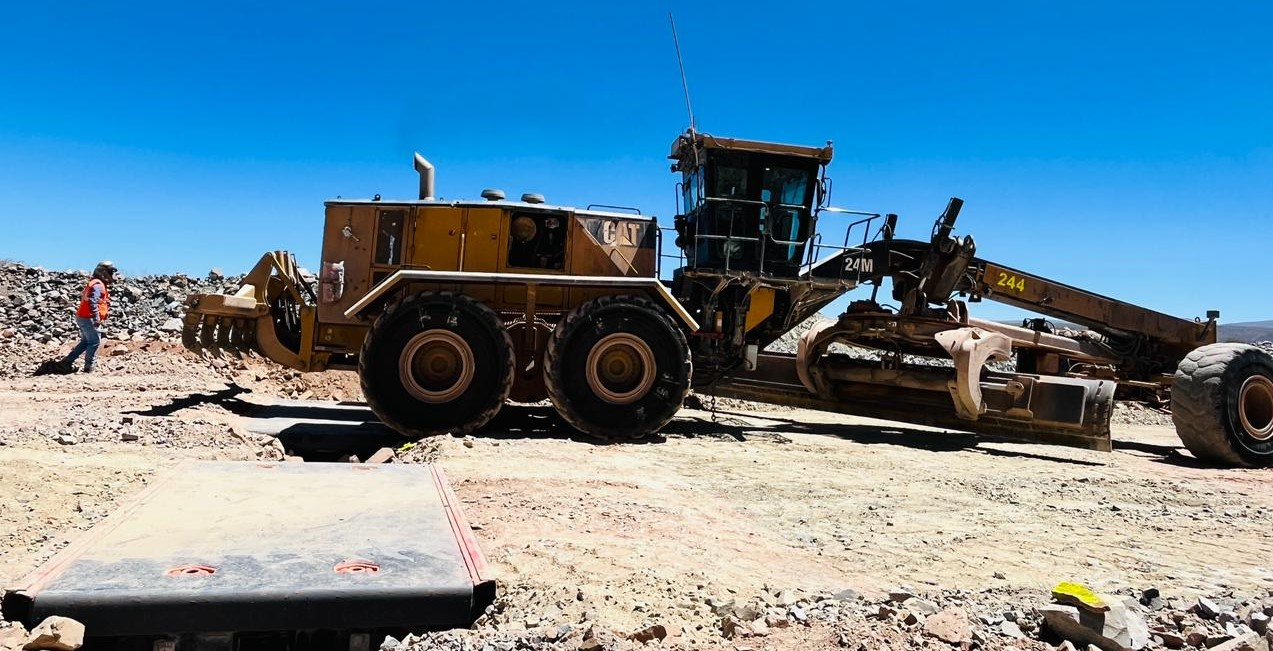
\includegraphics[width=0.85\textwidth]{figures_individual/raw_p03_img2_1273x651.png}
    \caption{Nivelación con la Motoniveladora CAT 24M (M244).}
\end{figure}

\begin{figure}[htbp]
    \centering
    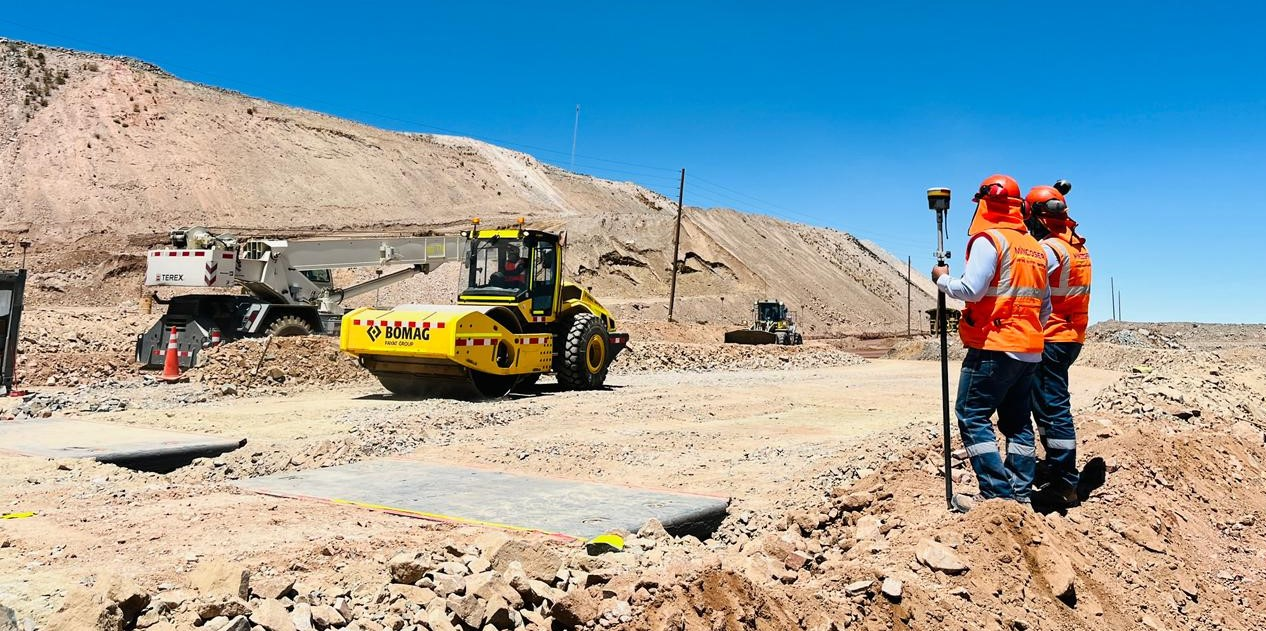
\includegraphics[width=0.85\textwidth]{figures_individual/raw_p03_img3_1266x631.png}
    \caption{Compactación con Rodillo Bomag y apoyo técnico de MINCOSER.}
\end{figure}

\subsection{Ubicación}
El área de pesaje estuvo delimitada por el parqueo Cocotea Bajo (Sur Oeste), Grifo Cocotea Bajo (Sur Este) y la Tranquera 4 (Norte). En la Figura 3 se muestra la ubicación del área del pesaje en el software MineOperate.

\begin{figure}[htbp]
    \centering
    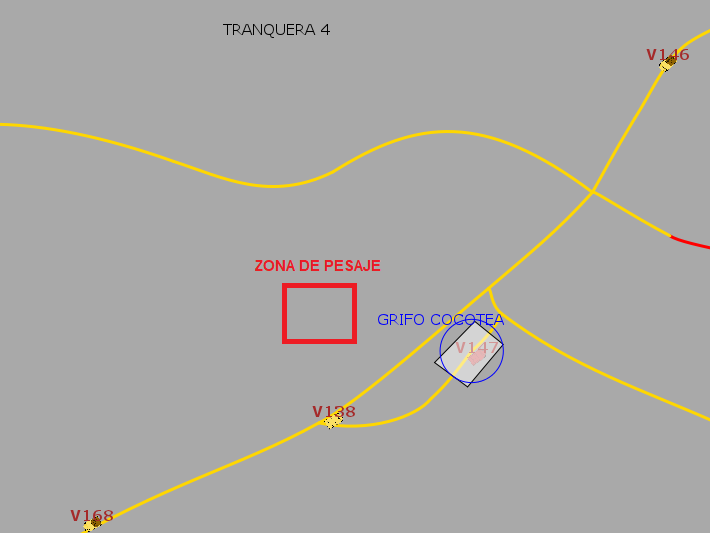
\includegraphics[width=0.85\textwidth]{figures_individual/raw_p04_img2_710x533.png}
    \caption{Ubicación de la zona de pesaje en software MineOperate.}
\end{figure}

\subsection{Personal a Cargo}
Durante la realización del pesaje participaron diversas áreas y empresas contratistas, según la Tabla 1 adjunta:

\begin{figure}[htbp]
    \centering
    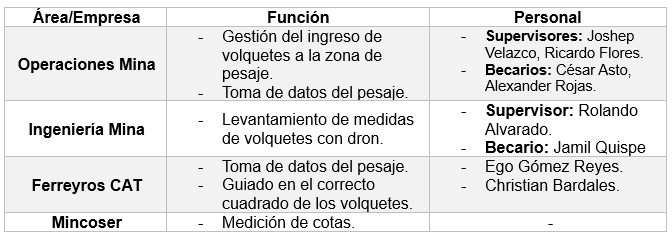
\includegraphics[width=0.90\textwidth]{figures_individual/raw_p04_img3_672x236.png}
    \caption{Funciones del personal a cargo del pesaje.}
\end{figure}

El trabajo tuvo una duración total de nueve (9) días, iniciando el 12 de octubre de 2025 y culminando el 20 de octubre de 2025. Durante la jornada final, y a solicitud de la empresa Ferreyros CAT, se realizaron repesajes de los volquetes V132, V144, V163 y V164, efectuándose dos mediciones por cada unidad en condición de carga.

\section{OBJETIVOS}
\begin{enumerate}[label=\alph*.]
    \item Determinar el peso vacío (EMW) y carga útil (Payload) de los 46 volquetes de Operaciones Mina Cuajone.
    \item Mostrar la distribución de peso (ton) en cada posición de los neumáticos.
    \item Cuantificar en toneladas, el impacto de los accesorios adicionales en la distribución del peso del volquete.
    \item Calcular la diferencia entre el tonelaje real (balanza) y el tonelaje de la pantalla de ADVISOR (Caterpillar) y Payload meter (Komatsu).
    \item Determinar los operadores de pala con mayor eficiencia en el centrado de carga.
\end{enumerate}

\section{PROCEDIMIENTO DEL PESAJE}
El área de pesaje, de 15 m de ancho por 30 m de largo, se ubicó en la ruta de descarga hacia el depósito de desmonte Cocotea Bajo. En la Figura 4 se muestra la ubicación de los PADs y el acceso a la balanza. Los volquetes ingresaron a los PADs a una velocidad máxima de 5 km/h para garantizar la estabilidad de la balanza durante la medición.

\begin{figure}[htbp]
    \centering
    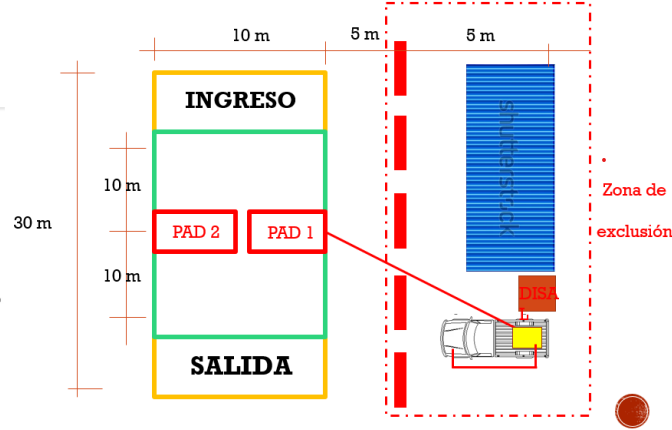
\includegraphics[width=0.85\textwidth]{figures_individual/raw_p05_img2_672x430.png}
    \caption{Vista en planta de la zona de pesaje y acceso a balanza PADs.}
\end{figure}

El pesaje de cada volquete se realizó tres (3) veces vacío y cuatro (4) veces cargado con desmonte. El requerimiento del fabricante indica que el cálculo del peso del volquete vacío (EMW), debe realizarse con los fluidos al 100\%, debido a ello cada volquete contó con al menos 90\% de combustible. En el pesaje cargado se mantuvo un mínimo de 50\% de combustible.

\subsection{Procedimiento de Pesaje Operacional}
\begin{enumerate}[label=\alph*.]
    \item Previa coordinación entre Control Mina y el becario de Operaciones Mina vía radial (frecuencia C2) para autorizar el ingreso de los volquetes.
    \item En la frecuencia 13 (local), y con apoyo del vigía, se brindan las indicaciones al operador del volquete para posicionar el eje delantero sobre ambos PADs.
    \item Una vez que los neumáticos del eje delantero se encuentran centrados y la lectura del pesómetro se estabiliza, se registran los datos en el formato establecido.
    \item Posteriormente, bajo las indicaciones del becario de Operaciones Mina, se posiciona el eje trasero sobre ambos PADs y se realiza el registro correspondiente.
    \item Finalmente, se indica al operador del volquete su salida de la zona de pesaje si se encuentra cargado; en caso de estar vacío, debe retornar inmediatamente a la zona de ingreso hasta completar sus 3 pasadas.
\end{enumerate}

\begin{figure}[htbp]
    \centering
    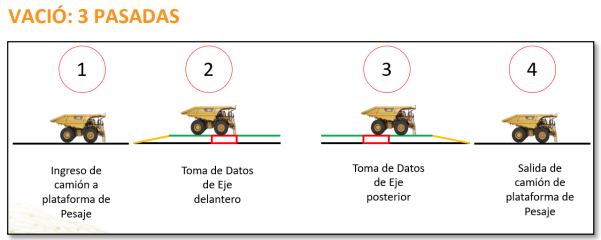
\includegraphics[width=0.80\textwidth]{figures_individual/raw_p06_img3_601x240.png}
    \caption{Procedimiento de pesaje del volquete vacío sobre PADs.}
\end{figure}

\begin{figure}[htbp]
    \centering
    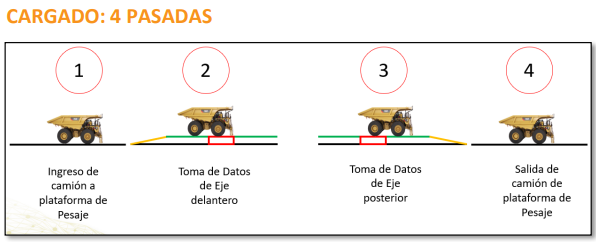
\includegraphics[width=0.80\textwidth]{figures_individual/raw_p06_img2_596x242.png}
    \caption{Procedimiento de pesaje del volquete cargado sobre PADs.}
\end{figure}

\section{DATOS RECOPILADOS}
\subsection{Datos Procesados}
Los datos registrados en campo correspondieron a: fecha y hora del pesaje, tipo de material transportado, asignación de pala y número de pases de carguío, condición cargado/vacío, lecturas de PADs en eje delantero y posterior (derecho e izquierdo), payload del volquete, tonelaje VIMS/Display, porcentaje de combustible y horómetro.

\subsection{Cálculo del Volquete Vacío y Cargado}
El cálculo del peso del volquete cargado y vacío se realizó mediante:
\begin{equation}
\text{Peso del eq.}_{\text{vacío/cargado}} = \text{ED}(\text{TI} + \text{TD}) + \text{EP}(\text{TI} + \text{TD})
\end{equation}
\noindent donde $\text{ED}$ es el eje delantero, $\text{EP}$ es el eje posterior, $\text{TI}$ es el tonelaje del PAD izquierdo y $\text{TD}$ es el tonelaje del PAD derecho.

El tonelaje correspondiente al combustible se determinó mediante:
\begin{equation}
\text{Toneladas de Combustible} = (\text{Capacidad volumétrica}) \cdot (\text{Densidad}) \cdot (\%\text{Combustible})
\end{equation}
\noindent con densidad del combustible diésel igual a .00322\text{ tn/gl}$.

\begin{figure}[htbp]
    \centering
    
\includegraphics[width=0.85\textwidth]{figures_individual/charts_v2/fig07_combustible.png}
    \caption{Capacidad volumétrica del tanque de combustible por modelo de volquete (Galones).}
\end{figure}

\section{ANÁLISIS DE PESO VACIO, CARGADO Y PAYLOAD}
\subsection{Flota Caterpillar 797F}
El volquete V144 destaca por ser el más ligero con 284 toneladas, debido a que su tolva es una Austin Westech, a diferencia de los demás volquetes que presentan una tolva Austin JEC. En promedio hay una variación de 14 toneladas entre ambos modelos de tolva.

\begin{figure}[htbp]
    \centering
    
\includegraphics[width=0.80\textwidth]{figures_individual/charts_v2/fig08_pesaje_797f.png}
    \caption{Pesaje de la flota CAT 797F.}
\end{figure}

\noindent\textbf{TOLVA AUSTIN JEC:} Ancho: 7.6 m $\mid$ Altura de carga: 7.4 m $\mid$ Cola: 4.8 m $\mid$ Espesor: 0.4 m $\mid$ Enclavamiento: 10\circ$ $\mid$ Peso: 43.6 t.

\begin{figure}[htbp]
    \centering
    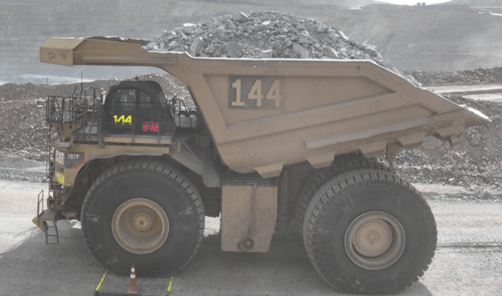
\includegraphics[width=0.75\textwidth]{figures_individual/raw_p08_img2_502x296.png}
    \caption{Tolva Austin JEC (Flota CAT 797F).}
\end{figure}

\noindent\textbf{TOLVA AUSTIN WESTECH:} Ancho: 7.7 m $\mid$ Altura de carga: 7.3 m $\mid$ Cola: 4.9 m $\mid$ Espesor: 0.4 m $\mid$ Enclavamiento: 8\circ$ $\mid$ Peso: 30.6 t.

\begin{figure}[htbp]
    \centering
    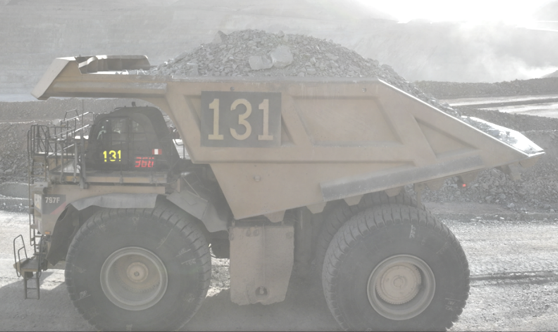
\includegraphics[width=0.75\textwidth]{figures_individual/raw_p08_img3_558x332.png}
    \caption{Tolva Austin WESTECH (Flota CAT 797F).}
\end{figure}

\subsection{Flota Caterpillar 798AC}
En la Figura 10 se muestra el resultado de pesaje de la flota CAT 798AC. En carga útil, el volquete V10 de tolva MP supera en 3 toneladas al volquete V11 de tolva HE. Estos volquetes no presentan parachoque.

\begin{figure}[htbp]
    \centering
    
\includegraphics[width=0.80\textwidth]{figures_individual/charts_v2/fig10_pesaje_798ac.png}
    \caption{Pesaje de la flota CAT 798AC.}
\end{figure}

\noindent\textbf{TOLVA MP (Max Payload):} Ancho: 9.93 m $\mid$ Altura de carga: 7.04 m $\mid$ Cola: 5.03 m $\mid$ Espesor: 0.4 m $\mid$ Enclavamiento: 12\circ$.
\begin{figure}[htbp]
    \centering
    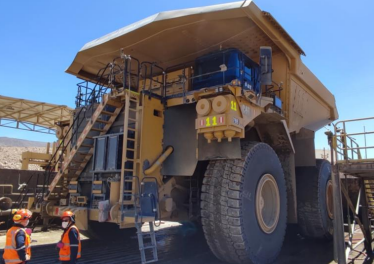
\includegraphics[width=0.70\textwidth]{figures_individual/raw_p09_img2_374x264.png}
    \caption{Tolva MP (Max Payload) -- CAT 798AC.}
\end{figure}

\noindent\textbf{TOLVA HE (High Efficiency):} Ancho: 9.74 m $\mid$ Altura de carga: 7.66 m $\mid$ Cola: 4.91 m $\mid$ Espesor: 0.44 m $\mid$ Enclavamiento: 16\circ$.
\begin{figure}[htbp]
    \centering
    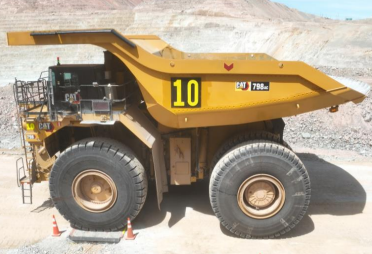
\includegraphics[width=0.70\textwidth]{figures_individual/raw_p09_img3_372x254.png}
    \caption{Tolva HE (High Efficiency) -- CAT 798AC.}
\end{figure}

\subsection{Flota Caterpillar 793D}
El peso del volquete V120 supera en 5 toneladas al volquete V121. El volquete V120 cargó en promedio 9 toneladas más que el V121.

\begin{figure}[htbp]
    \centering
    
\includegraphics[width=0.80\textwidth]{figures_individual/charts_v2/fig12_pesaje_793d.png}
    \caption{Pesaje de la flota CAT 793D.}
\end{figure}

\noindent\textbf{TOLVA MSDII (V120):} Estándar $\mid$ Ancho: 7.72 m $\mid$ Altura de carga: 6.41 m $\mid$ Cola: 4.35 m $\mid$ Espesor: 0.43 m $\mid$ Enclavamiento: 9\circ$.
\begin{figure}[htbp]
    \centering
    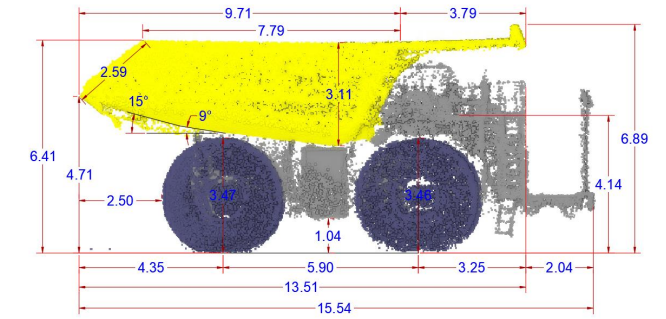
\includegraphics[width=0.75\textwidth]{figures_individual/raw_p09_img4_666x319.png}
    \caption{Tolva MSDII de 7.72 m (Volquete V120).}
\end{figure}

\noindent\textbf{TOLVA MSDII (V121):} Estándar $\mid$ Ancho: 7.44 m $\mid$ Altura de carga: 6.19 m $\mid$ Cola: 4.17 m $\mid$ Espesor: 0.44 m $\mid$ Enclavamiento: 13\circ$.
\begin{figure}[htbp]
    \centering
    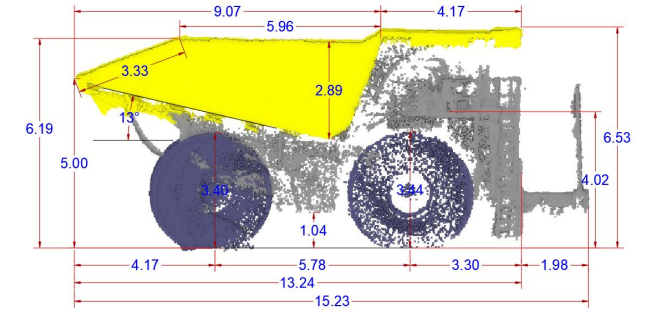
\includegraphics[width=0.75\textwidth]{figures_individual/raw_p09_img5_653x314.png}
    \caption{Tolva MSDII de 7.44 m (Volquete V121).}
\end{figure}

\subsection{Flota Komatsu 930E}
Los volquetes V100 y V101, equipados con tolvas DT-Hiload, presentan pesos vacíos con mínima variación (1 t). En su lugar, el V103 posee tolva Estándar, mientras que el V105 una Austin WESTECH. NOTA: Todos los volquetes presentan parachoque y ninguno protector de goma.

\begin{figure}[htbp]
    \centering
    
\includegraphics[width=0.80\textwidth]{figures_individual/charts_v2/fig14_pesaje_930e.png}
    \caption{Pesaje de la flota Komatsu 930E.}
\end{figure}

\noindent\textbf{TOLVA DT HILOAD:} Ancho: 8.66 m $\mid$ Altura de carga: 7.41 m $\mid$ Cola: 4.85 m $\mid$ Espesor: 0.26 m $\mid$ Enclavamiento: 13\circ$ $\mid$ Peso: 33.2 t.
\begin{figure}[htbp]
    \centering
    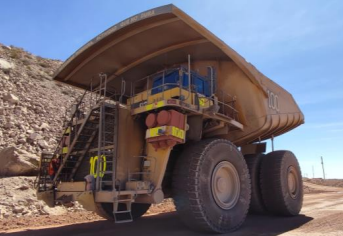
\includegraphics[width=0.70\textwidth]{figures_individual/raw_p10_img2_343x236.png}
    \caption{Tolva DT Hiload (Komatsu 930E).}
\end{figure}

\noindent\textbf{TOLVA AUSTIN WESTECH:} Ancho: 8.58 m $\mid$ Altura de carga: 7.47 m $\mid$ Cola: 4.6 m $\mid$ Espesor: 0.39 m $\mid$ Enclavamiento: 9\circ$ $\mid$ Peso: 39.5 t.
\begin{figure}[htbp]
    \centering
    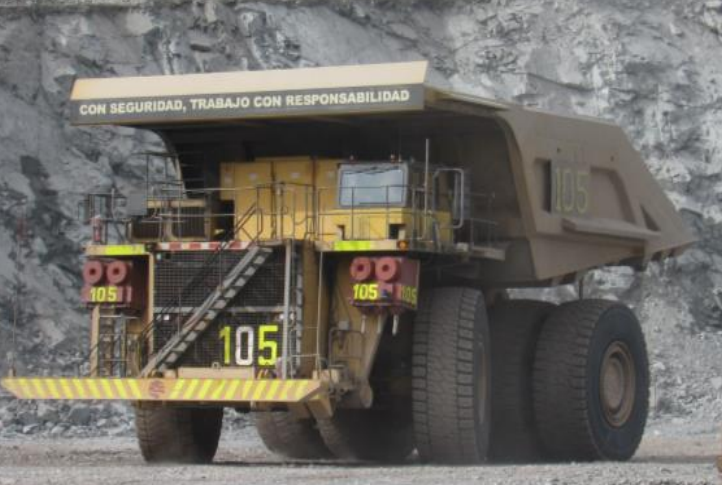
\includegraphics[width=0.75\textwidth]{figures_individual/raw_p10_img3_722x485.png}
    \caption{Tolva Austin WESTECH (Komatsu 930E).}
\end{figure}

\subsection{Flota Komatsu 930E-4}
\begin{figure}[htbp]
    \centering
    
\includegraphics[width=0.80\textwidth]{figures_individual/charts_v2/fig16_pesaje_930e4.png}
    \caption{Pesaje de la flota Komatsu 930E-4.}
\end{figure}

\noindent\textbf{TOLVA AUSTIN JEC (V110, V112):} Altura de carga: 7.28 m $\mid$ Cola: 4.71 m $\mid$ Espesor: 0.5 m $\mid$ Enclavamiento: 8\circ$ $\mid$ Peso: 35.5 t.
\begin{figure}[htbp]
    \centering
    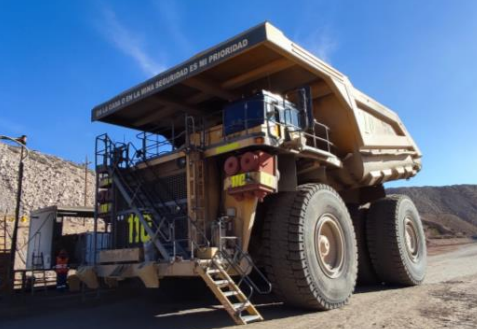
\includegraphics[width=0.75\textwidth]{figures_individual/raw_p10_img4_477x329.png}
    \caption{Tolva Austin JEC (Flota 930E-4).}
\end{figure}

\noindent\textbf{TOLVA ESTÁNDAR (V109, V111, V113):} Cola: 4.6 m $\mid$ Espesor: 0.39 m $\mid$ Enclavamiento: 9\circ$.
\begin{figure}[htbp]
    \centering
    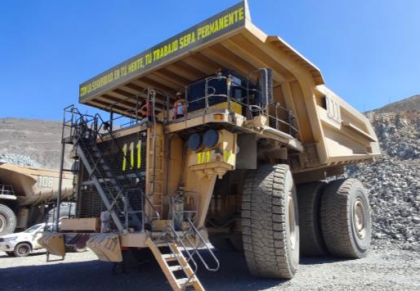
\includegraphics[width=0.75\textwidth]{figures_individual/raw_p10_img5_420x291.png}
    \caption{Tolva Estándar (Flota 930E-4).}
\end{figure}

\subsection{Flota Komatsu 930E-4SE}
En la flota 930E-4SE, el volquete V116 supera en 6 toneladas al volquete V115 en el eje trasero debido a dados instalados en su tolva DT Hiload Phase X.

\begin{figure}[htbp]
    \centering
    
\includegraphics[width=0.80\textwidth]{figures_individual/charts_v2/fig18_pesaje_930e4se.png}
    \caption{Pesaje de la flota Komatsu 930E-4SE.}
\end{figure}

\begin{figure}[htbp]
    \centering
    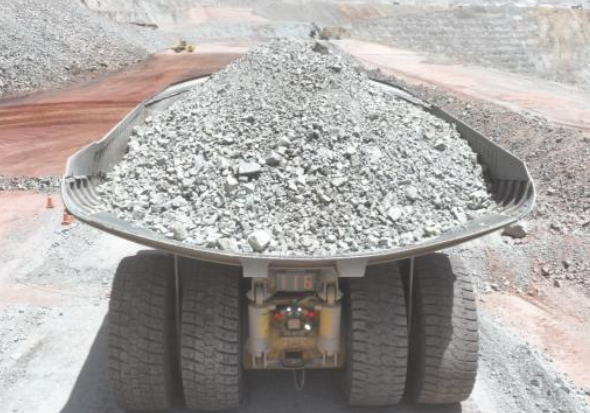
\includegraphics[width=0.70\textwidth]{figures_individual/raw_p11_img2_590x413.png}
    \caption{Volquete V115 sin dados.}
\end{figure}

\begin{figure}[htbp]
    \centering
    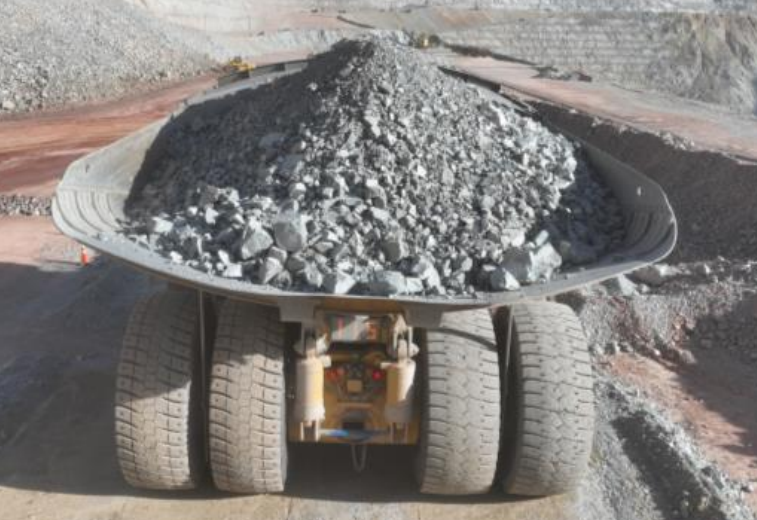
\includegraphics[width=0.75\textwidth]{figures_individual/raw_p11_img3_757x520.png}
    \caption{Volquete V116 con dados instalados.}
\end{figure}

\subsection{Flota Komatsu 980E-4}
El menor peso vacío (EMW) de los volquetes V160 y V165 se debe a que no tienen instaladas gomas de protección (liner). En promedio hay una diferencia de 15 toneladas en comparación a los volquetes que presentan liner.

\begin{figure}[htbp]
    \centering
    
\includegraphics[width=0.85\textwidth]{figures_individual/charts_v2/fig20_pesaje_980e4.png}
    \caption{Pesaje de la flota Komatsu 980E-4.}
\end{figure}

\subsection{Flota Komatsu 980E-5}
\begin{figure}[htbp]
    \centering
    
\includegraphics[width=0.80\textwidth]{figures_individual/charts_v2/fig21_pesaje_980e5.png}
    \caption{Pesaje de la flota Komatsu 980E-5.}
\end{figure}

\begin{figure}[htbp]
    \centering
    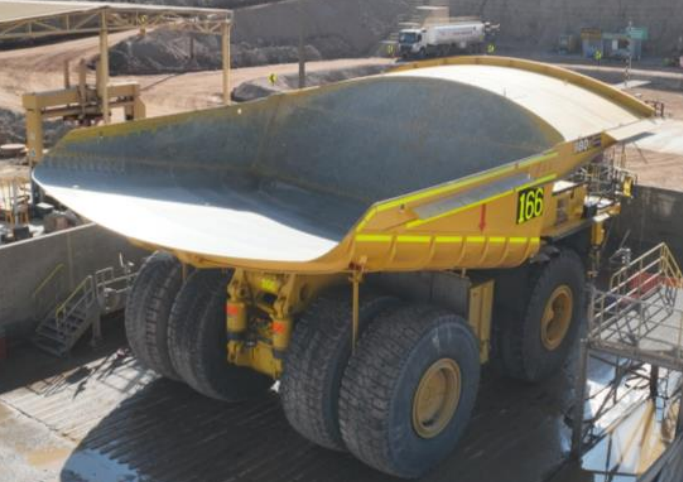
\includegraphics[width=0.75\textwidth]{figures_individual/raw_p12_img3_683x482.png}
    \caption{Modelo de tolva DT Hiload Phase X (Flota 980E-5).}
\end{figure}

\begin{figure}[htbp]
    \centering
    
\includegraphics[width=0.85\textwidth]{figures_individual/charts_v2/fig23_distrib_pos12_vacio.png}
    \caption{Análisis de distribución en la posición 1 y 2 vacío.}
\end{figure}

\section{DISTRIBUCIÓN DE CARGA EN EL EJE DELANTERO}
\subsection{Flota de Mayor Capacidad de Tonelaje}
En la flota CAT 797F y CAT 798AC hay un desbalance de 7.5 toneladas entre la posición 1 y 2 en vacío. En condición de carga, la posición 1 y 2 cargan en promedio 115 toneladas, con picos de hasta 134 toneladas, superando excesivamente el target de Michelin (109 toneladas) en el tamaño 59/80R63 y al target de Bridgestone VREV (123.5 toneladas). Esto se agrava en la rampa negativa de la ruta de P08 hacia Cuajone Este.

\begin{figure}[htbp]
    \centering
    
\includegraphics[width=0.85\textwidth]{figures_individual/charts_v2/fig24_distrib_pos12_cargado.png}
    \caption{Análisis de distribución de peso en la posición 1 y 2 cargado.}
\end{figure}

\subsection{Flota de Menor Capacidad de Tonelaje}
\begin{figure}[htbp]
    \centering
    
\includegraphics[width=0.85\textwidth]{figures_individual/charts_v2/fig25_distrib_pos12_vacio_menor.png}
    \caption{Análisis de distribución de peso en posición 1 y 2 vacío (Menor tonelaje).}
\end{figure}

\section{DISTRIBUCIÓN DE CARGA EN EL EJE POSTERIOR}
\begin{figure}[htbp]
    \centering
    
\includegraphics[width=0.85\textwidth]{figures_individual/charts_v2/fig26_distrib_post_cargado.png}
    \caption{Análisis de distribución de peso en posición 3\&4 vs 5\&6 cargado.}
\end{figure}

\begin{figure}[htbp]
    \centering
    
\includegraphics[width=0.85\textwidth]{figures_individual/charts_v2/fig27_distrib_post_vacio.png}
    \caption{Análisis de distribución de peso en posición 3\&4 vs 5\&6 vacío.}
\end{figure}

\begin{figure}[htbp]
    \centering
    
\includegraphics[width=0.85\textwidth]{figures_individual/charts_v2/fig28_distrib_post_cargado_menor.png}
    \caption{Distribución de peso en posición 3\&4 vs 5\&6 cargado (Menor tonelaje).}
\end{figure}

\begin{figure}[htbp]
    \centering
    
\includegraphics[width=0.85\textwidth]{figures_individual/charts_v2/fig29_distrib_post_vacio_menor.png}
    \caption{Distribución de peso en posición 3\&4 vs 5\&6 vacío (Menor tonelaje).}
\end{figure}

\section{DISTRIBUCIÓN DE CARGA POR EJE}
\begin{figure}[htbp]
    \centering
    
\includegraphics[width=0.85\textwidth]{figures_individual/charts_v2/fig30_distrib_eje_vacio_flota.png}
    \caption{Distribución de carga por eje en vacío (Flota mayor).}
\end{figure}

\begin{figure}[htbp]
    \centering
    
\includegraphics[width=0.85\textwidth]{figures_individual/charts_v2/fig31_distrib_eje_vacio_flota2.png}
    \caption{Distribución de carga por eje en vacío (Flota menor).}
\end{figure}

\begin{figure}[htbp]
    \centering
    
\includegraphics[width=0.85\textwidth]{figures_individual/charts_v2/fig32_distrib_eje_cargado_flota.png}
    \caption{Distribución de carga por eje en condición de carga.}
\end{figure}

\section{PALEROS CON MAYOR EFICIENCIA EN EL CENTRADO DE CARGA}
Los operadores Oscar Pinedo, Efraín Huaypuna y Edil Valdivia destacan con la mayor eficiencia en la distribución de carga.

\begin{figure}[htbp]
    \centering
    
\includegraphics[width=0.85\textwidth]{figures_individual/charts_v2/fig49_ranking_paleros.png}
    \caption{Ranking de operadores con mejor eficiencia en la distribución de carga.}
\end{figure}

\section{PAYLOAD VS TONELAJE VIMS / PLM}
El tonelaje de la pantalla VIMS en el volquete V11 es mayor en 1.6\% que la carga real. En la flota CAT 793D, en el volquete V121 el sistema VIMS marca un 4.4\% menos respecto a la carga útil real. En la flota Komatsu 980 la variación entre el tonelaje Payload Meter y el payload real varía en más de 5\% en los volquetes V163, V164 y V165.

\begin{figure}[htbp]
    \centering
    
\includegraphics[width=0.85\textwidth]{figures_individual/charts_v2/fig54_vims_980e.png}
    \caption{Tonelaje VIMS vs Payload Komatsu 980E.}
\end{figure}

\section{CÁLCULO DEL PESO DEL PARACHOQUE}
El volquete V131 fue pesado 6 veces vacío: 3 veces sin parachoques y 3 veces con parachoques instalado el 15 de octubre del 2025. El primer pesaje fue con .61\%$ de combustible y el segundo a .00\%$.

\begin{equation}
\text{Peso Total}_1 = \text{Peso Vacío} + \text{Combustible}_1
\end{equation}
\begin{equation}
\text{Peso Total}_2 = \text{Peso Vacío} + \text{Combustible}_2 + \text{Parachoques}
\end{equation}
\begin{equation}
\text{Parachoque (t)} = \text{Peso Total}_2 - \text{Peso Total}_1 - \text{Combustible}_2 + \text{Combustible}_1
\end{equation}
\begin{equation}
\text{Parachoque (t)} = 299.30\text{ t} - 296.93\text{ t} - 94.00\%(T) + 92.61\%(T) = 2.37\text{ t} - 1.39\%(T)
\end{equation}
\begin{equation}
\text{Parachoque (t)} = 2.37\text{ t} - (1.39\% \times 2,000\text{ gl} \times 3.22\text{ kg/gl}) = 2.30\text{ t}
\end{equation}

\section{CONCLUSIONES}
\begin{enumerate}[label=\arabic*.]
    \item El tonelaje añadido por la instalación del parachoques en los volquetes CATERPILLAR 797F le añade 2.3 toneladas al eje delantero.
    \item El tonelaje añadido al eje posterior por la instalación del liner en la flota KOMATSU 980E-4 significa un adicional de 15 toneladas.
    \item Los operadores de pala con mejor centrado de carga son Oscar Pinedo, Efraín Huaypuna y Edil Valdivia.
    \item En la flota CATERPILLAR 798 AC, el volquete V10 de tolva MP presenta 3 toneladas más de carga útil que el volquete V11 de tolva HE.
    \item En condición vacía, en las flotas CAT 797F y CAT 798AC existe un desbalance de más de 7 toneladas entre los neumáticos del eje delantero, debido a la ubicación del tanque de combustible.
    \item En condición de carga, los neumáticos de posición 1 de la flota CAT 797F soportan más de 115 toneladas, excediendo el target de Michelin en el tamaño 59/80R63 (109 t).
    \item Se debe inspeccionar las suspensiones y/o las unidades de tonelajes del sistema Payload Meter en los volquetes V108, V115, V112, V165, V163, V164 y V165.
\end{enumerate}

\end{document}
